%%%%%%%%%%%%%%%%%% DERIVATIVES 1D%%%%%%%%%%%%%%%%%%

\newcommand{\FirstDerivative}[1]
{
	%\onegrapht{ xlabel = $x$, ylabel = $u_x(x)$, no marks, xmax = 1, xmin = -1}
	%
	%{./doc/chapters/Finite_Differences/figures/Ux1D.plt}{ }{1}{ #1 }
	\onegraph{$x$}{$\dv*{u}{x}$}{ no marks, xmax = 1, xmin = -1}
	%
	{./doc/chapters/Finite_Differences/figures/Ux1D.plt}{ }{1}{ #1 }
}



\newcommand{\SecondDerivative}[1]
{
	%\onegrapht{ xlabel = $x$, ylabel = $u_{xx}(x)$, no marks, xmax = 1, xmin = -1}
	%
	%{./doc/chapters/Finite_Differences/figures/Uxx1D.plt}{ }{1}{ #1 }
	\onegraph{$x$}{$\dv*[2]{u}{x}$}{ no marks, xmax = 1, xmin = -1}
	%
	{./doc/chapters/Finite_Differences/figures/Uxx1D.plt}{ }{1}{ #1 }
}
	


\newcommand{\FirstDerivativeError}[1]
{
	%\onegrapht{ xlabel = $x$, ylabel = $E(x)$, no marks, xmax = 1, xmin = -1}
	%
	%{./doc/chapters/Finite_Differences/figures/Ux1D.plt}{ }{2}{ #1 }
	\onegraph{$x$}{$E(x)$}{ no marks, xmax = 1, xmin = -1}
	%
	{./doc/chapters/Finite_Differences/figures/Ux1D.plt}{ }{2}{ #1 }
}



\newcommand{\SecondDerivativeError}[1]
{
	%\onegrapht{ xlabel = $x$, ylabel = $E(x)$, no marks, xmax = 1, xmin = -1}
	%
	%{./doc/chapters/Finite_Differences/figures/Uxx1D.plt}{ }{2}{ #1 }
	\onegraph{$x$}{$E(x)$}{ no marks, xmax = 1, xmin = -1}
	%
	{./doc/chapters/Finite_Differences/figures/Uxx1D.plt}{ }{2}{ #1 }
}


%%%%%%%%%%%%%%%%%% DERIVATIVES 2D%%%%%%%%%%%%%%%%%%

\newcommand{\Uxx}[1]
{   
	\onecontour{ xlabel = $x$, ylabel = $y$, colormap/bluered}{21}
	%
	{./doc/chapters/Finite_Differences/figures/Uxx.dat}{}{ #1 }
}

\newcommand{\ErrorUxx}[1]
{   
	\onecontour{ xlabel = $x$, ylabel = $y$, colormap/bluered}{21}
	%
	{./doc/chapters/Finite_Differences/figures/ErrorUxx.dat}{}{ #1 }
}

\newcommand{\Uxy}[1]
{   
	\onecontour{ xlabel = $x$, ylabel = $y$, colormap/bluered}{21}
	%
	{./doc/chapters/Finite_Differences/figures/Uxy.dat}{}{ #1 }
}

\newcommand{\ErrorUxy}[1]
{   
	\onecontour{ xlabel = $x$, ylabel = $y$, colormap/bluered}{21}
	%
	{./doc/chapters/Finite_Differences/figures/ErrorUxy.dat}{}{ #1 }
}

%%%%%%%%%%%%%%%%%% TRUNCATION AND ROUND OFF ERROR %%%%%%%%%%%%%%%%%%

\newcommand{\ErrorqTwoBoundary}[1]
{

	\onegraph{$\log \Delta x$}{$\log E(x)$}{ no marks, xmax = -2.3, xmin= -9.2}
	%
	{./doc/chapters/Finite_Differences/figures/Derivative_error/N=0/Derivative_error.dat}{ }{1}{ #1 }
}

\newcommand{\ErrorqFourBoundary}[1]
{

	\onegraph{$\log \Delta x$}{$\log E(x)$}{ no marks, xmax = -2.3, xmin= -9.2}
	%
	{./doc/chapters/Finite_Differences/figures/Derivative_error/N=0/Derivative_error.dat}{ }{2}{ #1 }
}

\newcommand{\ErrorqSixBoundary}[1]
{

	\onegraph{$\log \Delta x$}{$\log E(x)$}{ no marks, xmax = -2.3, xmin= -9.2}
	%
	{./doc/chapters/Finite_Differences/figures/Derivative_error/N=0/Derivative_error.dat}{ }{3}{ #1 }
}

\newcommand{\ErrorqEightBoundary}[1]
{
	\onegraph{$\log \Delta x$}{$\log E(x)$}{ no marks, xmax = -2.3, xmin= -9.2}
	%
	{./doc/chapters/Finite_Differences/figures/Derivative_error/N=0/Derivative_error.dat}{ }{4}{ #1 }
}




\newcommand{\ErrorqTwoMiddle}[1]
{
	\onegraph{$\log \Delta x$}{$\log E(x)$}{ no marks, xmax = -2.3, xmin= -9.2}
	%
	{./doc/chapters/Finite_Differences/figures/Derivative_error/N=N2/Derivative_error.dat}{ }{1}{ #1 }
}

\newcommand{\ErrorqFourMiddle}[1]
{
	\onegraph{$\log \Delta x$}{$\log E(x)$}{ no marks, xmax = -2.3, xmin= -9.2}
	%
	{./doc/chapters/Finite_Differences/figures/Derivative_error/N=N2/Derivative_error.dat}{ }{2}{ #1 }
}

\newcommand{\ErrorqSixMiddle}[1]
{
	\onegraph{$\log \Delta x$}{$\log E(x)$}{ no marks, xmax = -2.3, xmin= -9.2}
	%
	{./doc/chapters/Finite_Differences/figures/Derivative_error/N=N2/Derivative_error.dat}{ }{3}{ #1 }
}

\newcommand{\ErrorqEightMiddle}[1]
{
	\onegraph{$\log \Delta x$}{$\log E(x)$}{ no marks, xmax = -2.3, xmin= -9.2}
	%
	{./doc/chapters/Finite_Differences/figures/Derivative_error/N=N2/Derivative_error.dat}{ }{4}{ #1 }
}



%%%%%%%%%%%%%%%%%% BVP 1D %%%%%%%%%%%%%%%%%%


\newcommand{\UBVPONED}[1]
{
	\onegraph{$x$}{$u(x)$}{ no marks, xmax = 1, xmin= -1}
	%
	{./doc/chapters/Finite_Differences/figures/BVP1D.plt}{ }{1}{ #1 }
}


\newcommand{\ERRORUBVPONED}[1]
{
	\onegraph{$x$}{$E(x)$}{ no marks, xmax = 1, xmin= -1}
	%
	{./doc/chapters/Finite_Differences/figures/BVP1D.plt}{ }{2}{ #1 }
}




%\include{./figures/VanDerPool}

\newcommand{\stencilpt}[4]
{
	\node[circle,fill,draw,inner sep=1.5pt,label={#4},#1] at (#2) (#3) {}
}

\newcommand{\ABMStencil}[1]
{
	\vspace{0.5cm}
	\begin{center}
		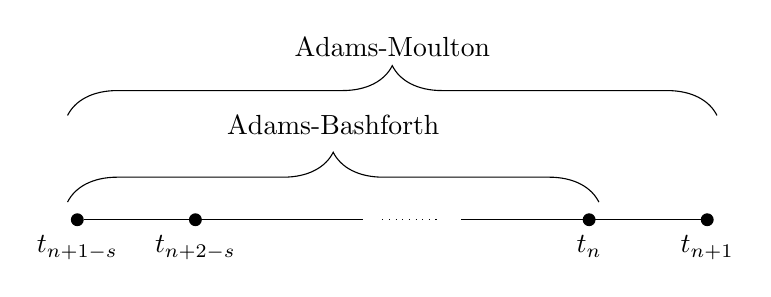
\begin{tikzpicture}
			\stencilpt{}{-4,0}{tn+1-s}{below:$t_{n+1-s}$};
			\stencilpt{}{-2.5,0}{un1}{below:$t_{n+2-s}$};
			
			\node at (-0.25,0)(Intermediate1) {};
			\node at (0.75,0)(Intermediate2) {};
				
			\stencilpt{}{2.5,0}{tn}{below:$t_{n}$};	
			\stencilpt{}{4,0}{tn+1}{below:$t_{n+1}$};
			
			\draw[](tn+1-s)	-- (Intermediate1);
			\draw[dotted](Intermediate1) -- (Intermediate2);
			\draw[](Intermediate2)	-- (tn+1);
			
			\node at (-4,0.1)(LeftABBrace) {};
			\node at (2.5,0.1)(RightABBrace) {};
			\draw [xscale=1/12, decoration={brace, amplitude=18pt},decorate] (LeftABBrace.north west) -- node [pos=0.5,midway] {} 
			(RightABBrace.north east);
			\node at (-0.75,1.2)(AB) {Adams-Bashforth};
			
			\node at (-4,1.2)(LeftAMBrace) {};
			\node at (4,1.2)(RightAMBrace) {};
			\draw [xscale=1/12, decoration={brace, amplitude=18pt},decorate] (LeftAMBrace.north west) -- node [pos=0.5,midway,yshift=0.1cm] 
			{} (RightAMBrace.north east);
			\node at (0,2.2)(AB) {Adams-Moulton};
		\end{tikzpicture}
	\end{center}
}




\newcommand{\MultivalueABMStencil}[1]
{
	\vspace{0.5cm}
	\begin{center}
		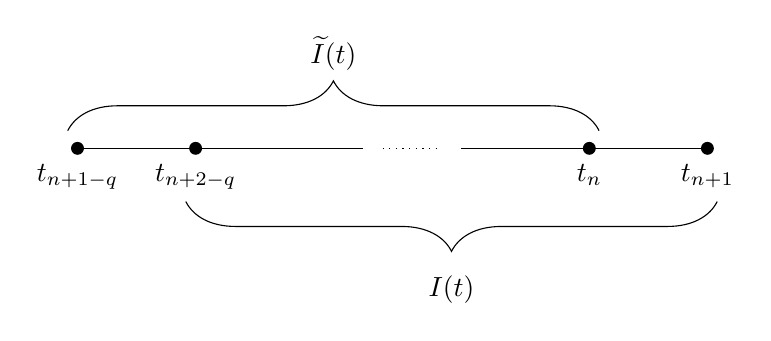
\begin{tikzpicture}
			\stencilpt{}{-4,0}{tn+1-q}{below:$t_{n+1-q}$};
			\stencilpt{}{-2.5,0}{un1}{below:$t_{n+2-q}$};
			
			\node at (-0.25,0)(Intermediate1) {};
			\node at (0.75,0)(Intermediate2) {};
			
			\stencilpt{}{2.5,0}{tn}{below:$t_{n}$};	
			\stencilpt{}{4,0}{tn+1}{below:$t_{n+1}$};
			
			\draw[](tn+1-q)	-- (Intermediate1);
			\draw[dotted](Intermediate1) -- (Intermediate2);
			\draw[](Intermediate2)	-- (tn+1);
			
			\node at (-4,0.1)(LeftABBrace) {};
			\node at (2.5,0.1)(RightABBrace) {};
			\draw [xscale=1/12, decoration={brace, amplitude=18pt},decorate] (LeftABBrace.north west) -- node [pos=0.5,midway] {} 
			(RightABBrace.north east);
			\node at (-0.75,1.2)(AB) {$\widetilde{ \vect{I}}(t)$};
			
			\node at (-2.5,-0.8)(LeftAMBrace) {};
			\node at 
			(4,-0.8)(RightAMBrace) {};
			\draw [xscale=1/12, decoration={brace, amplitude=18pt,mirror},decorate] (LeftAMBrace.north west) -- node 
			[pos=0.5,midway,yshift=0.1cm] {} (RightAMBrace.north east);
			\node at (0.75,-1.8)(AM) {$\vect{I}(t)$};
		\end{tikzpicture}
	\end{center}
}


%%%%%%%%%%%%%%%%%%%%%%%%%%%%%%%%%%%%%%%%%%%%%% DEVELOPER FIGURES


\newcommand{\EvenStencil}
{   
	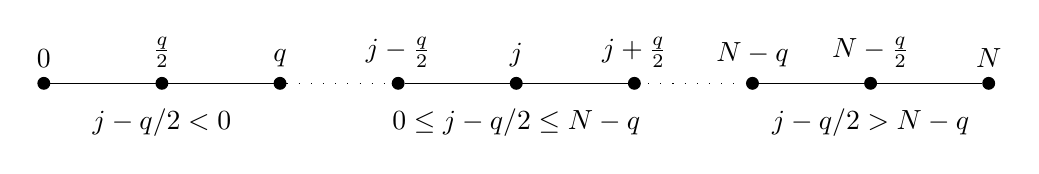
\begin{tikzpicture}
	
	%%% Stencil [ 0,q ]
	\stencilpt{}{-3,2}{0}{$0$};
	\stencilpt{}{-1.5,2}{q/2}{$\frac{q}{2}$};
	\stencilpt{}{0,2}{q}{$q$};
	\draw (0) -- (q);
	
	%%% Stencil [ j-q/2,j+q/2 ]
	\stencilpt{}{1.5,2}{j-q/2}{$j-\frac{q}{2}$};
	\stencilpt{}{3,2}{j}{$j$};	
	\stencilpt{}{4.5,2}{j+q/2}{$j+\frac{q}{2}$};
	\draw (j-q/2) -- (j+q/2);
	
	%%% Stencil [ N-q, N ]
	\stencilpt{}{6,2}{N-q}{$N-q$};
	\stencilpt{}{7.5,2}{N-q/2}{$N-\frac{q}{2}$};
	\stencilpt{}{9,2}{N}{$N$};
	\draw (N-q) -- (N);
	
	%%%%%%%%%DOTS BETWEEN STENCILS %%%%%%%%%%%%
	
	\draw[loosely dotted] (q) -- (j-q/2);
	\draw[loosely dotted] (j-q/2) -- (N-q/2);
	
	
	%%%%%%%%% STENCIL CONDITIONS
	\node(Stencil1) at (-1.5,1.5) {$j-q/2<0$};
	\node(Stencil2) at (3,1.5) {$0\leq j-q/2\leq N-q$};
	\node(Stencil3) at (7.5,1.5) {$j-q/2 > N-q$};
	\end{tikzpicture}
	
}


\newcommand{\OddStencil}%[1]
{   
	\begin{tikzpicture}
	%%% Stencil [ 0,q ]
	\stencilpt{}{-3,2}{0}{$0$};
	\stencilpt{}{-1.5,2}{q-1/2}{$\frac{q-1}{2}$};
	\stencilpt{}{0,2}{q}{$q$};
	
	\draw
	(0) -- (q);
	
	\stencilpt{}{1.5,2}{j-q-1/2}{$j-\frac{q-1}{2}$};
	\stencilpt{}{3,2}{j}{$j$};	
	\stencilpt{}{4.5,2}{j+q+1/2}{$j+\frac{q+1}{2}$};
	
	\draw
	(j-q-1/2) -- (j+q+1/2);
	
	\draw[loosely dotted]
	(q) -- (j-q/2);
	
	\stencilpt{}{6,2}{N-q}{$N-q$};
	\stencilpt{}{7.5,2}{N-q-1/2}{$N-\frac{q-1}{2}$};
	\stencilpt{}{9,2}{N}{$N$};
	\draw
	(N-q) -- (N);
	
	\draw[loosely dotted]
	(j-q/2) -- (N-q/2);
	
	
	
	%%%%%%%%% STENCIL CONDITIONS
	\node(Stencil1) at (-1.5,1.5) {$j-(q-1)/2<0$};
	\node(Stencil2) at (3,1.5) {$0\leq j-(q-1)/2\leq N-q$};
	\node(Stencil3) at (7.5,1.5) {$j-(q-1)/2 > N-q$};
	\end{tikzpicture}
	
}







    